
\chapter{Design of Module \textit{userprog}}


\section{Process Termination Messages \& Argument passing}

    \subsection{Initial Functionality}

	At the beginning of this project ... .

    \subsection{Data Structures and Functions}

    \begin{lstlisting}

      "In ... :"
	
	struct structure_def {
	    type field;
	};

	/* comments */
	variable definition;

	/* comments */
	function definition;

    \end{lstlisting}


    \subsection{Functionality}

	Function x works like this ... : (picture with sequence diagram or algorithm. See commented examples for including images or describing algorithms below)

    %\begin{figure}[h]
    %	\centering
    %	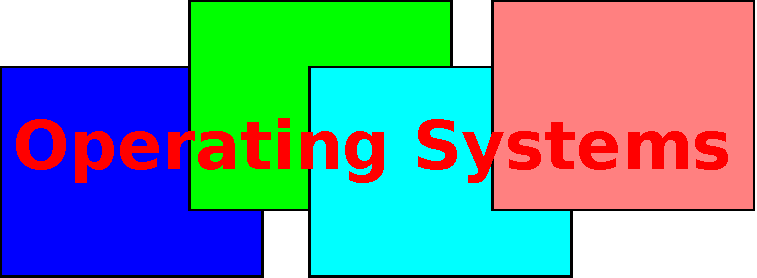
\includegraphics[width=0.5\textwidth]{figures/sample-image.pdf}
    %	\caption{Sample image}
    %	\label{fig:sample-image}
    %\end{figure}


    %Here you have a pseudo-code description of an algorithm taken fom \\ \href{http://en.wikibooks.org/wiki/LaTeX/Algorithms\_and\_Pseudocode\#Typesetting\_using\_the\_program\_package}{http://en.wikibooks.org/wiki/LaTeX}. It uses the \textit{program} package. Alternatively, you can use \textit{algorithmic} or \textit{algorithm2e} packages. 

    %\begin{program}
    %\mbox{Example of a pseudo-code algorithm description:}
    %\BEGIN %
    %  \FOR i:=1 \TO 10 \STEP 1 \DO
    %     |expt|(2,i); \\ |newline|() \OD %
    %\rcomment{This text will be set flush to the right margin}
    %\WHERE
    %\PROC |expt|(x,n) \BODY
    %          z:=1;
    %          \DO \IF n=0 \THEN \EXIT \FI;
    %             \DO \IF |odd|(n) \THEN \EXIT \FI;
    %\COMMENT{This is a comment statement};
    %                n:=n/2; x:=x*x \OD;
    %             \{ n>0 \};
    %             n:=n-1; z:=z*x \OD;
    %          |print|(z) \ENDPROC
    %\END
    %\end{program}


    \subsection{Design Decisions}

	This solution has the advantage that ... 

	On the other hand it is not so good that ... . 

	A better solution would be ... . 

	However, this solution is better than ...

    \subsection{Tests}

    \textbf{name of the test}\\
    \textit{Source:} path/to/test.c\\
    \textit{Purpose:} What does it check?\\
    \textit{Description:} Short description.
    \textit{Solution:(if necessary)} Here, if what the test does is something that was not explicitly asked in the requirements, it would be good to say that we already treat that situation and where. If it's something that should be solved only by the implementation of the requirements you can say: Solved by requirements fulfillment.
    
\section{System calls}

    \subsection{Initial Functionality}

	At the beginning of this project ... .

    \subsection{Data Structures and Functions}

    \begin{lstlisting}

      "In ... :"
	
	struct structure_def {
	    type field;
	};

	/* comments */
	variable definition;

	/* comments */
	function definition;

    \end{lstlisting}


    \subsection{Functionality}

	Function x works like this ... : (picture with sequence diagram or algorithm. See commented examples for including images or describing algorithms below)

    %\begin{figure}[h]
    %	\centering
    %	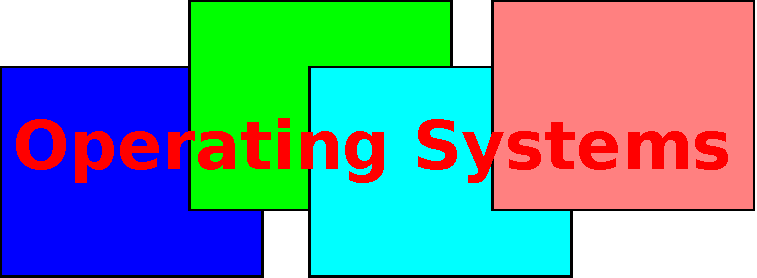
\includegraphics[width=0.5\textwidth]{figures/sample-image.pdf}
    %	\caption{Sample image}
    %	\label{fig:sample-image}
    %\end{figure}


    %Here you have a pseudo-code description of an algorithm taken fom \\ \href{http://en.wikibooks.org/wiki/LaTeX/Algorithms\_and\_Pseudocode\#Typesetting\_using\_the\_program\_package}{http://en.wikibooks.org/wiki/LaTeX}. It uses the \textit{program} package. Alternatively, you can use \textit{algorithmic} or \textit{algorithm2e} packages. 

    %\begin{program}
    %\mbox{Example of a pseudo-code algorithm description:}
    %\BEGIN %
    %  \FOR i:=1 \TO 10 \STEP 1 \DO
    %     |expt|(2,i); \\ |newline|() \OD %
    %\rcomment{This text will be set flush to the right margin}
    %\WHERE
    %\PROC |expt|(x,n) \BODY
    %          z:=1;
    %          \DO \IF n=0 \THEN \EXIT \FI;
    %             \DO \IF |odd|(n) \THEN \EXIT \FI;
    %\COMMENT{This is a comment statement};
    %                n:=n/2; x:=x*x \OD;
    %             \{ n>0 \};
    %             n:=n-1; z:=z*x \OD;
    %          |print|(z) \ENDPROC
    %\END
    %\end{program}


    \subsection{Design Decisions}

	This solution has the advantage that ... 

	On the other hand it is not so good that ... . 

	A better solution would be ... . 

	However, this solution is better than ...

    \subsection{Tests}

    \textbf{name of the test}\\
    \textit{Source:} path/to/test.c\\
    \textit{Purpose:} What does it check?\\
    \textit{Description:} Short description.
    \textit{Solution:(if necessary)} Here, if what the test does is something that was not explicitly asked in the requirements, it would be good to say that we already treat that situation and where. If it's something that should be solved only by the implementation of the requirements you can say: Solved by requirements fulfillment.
	

\section{Denying writes to executables}

     \subsection{Initial Functionality}

	At the beginning of this project ... .

    \subsection{Data Structures and Functions}

    \begin{lstlisting}

      "In ... :"
	
	struct structure_def {
	    type field;
	};

	/* comments */
	variable definition;

	/* comments */
	function definition;

    \end{lstlisting}


    \subsection{Functionality}

	Function x works like this ... : (picture with sequence diagram or algorithm. See commented examples for including images or describing algorithms below)

    %\begin{figure}[h]
    %	\centering
    %	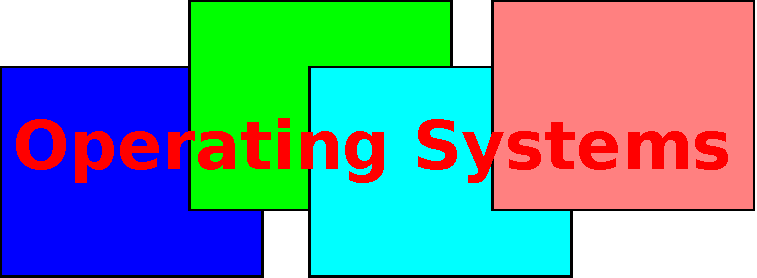
\includegraphics[width=0.5\textwidth]{figures/sample-image.pdf}
    %	\caption{Sample image}
    %	\label{fig:sample-image}
    %\end{figure}


    %Here you have a pseudo-code description of an algorithm taken fom \\ \href{http://en.wikibooks.org/wiki/LaTeX/Algorithms\_and\_Pseudocode\#Typesetting\_using\_the\_program\_package}{http://en.wikibooks.org/wiki/LaTeX}. It uses the \textit{program} package. Alternatively, you can use \textit{algorithmic} or \textit{algorithm2e} packages. 

    %\begin{program}
    %\mbox{Example of a pseudo-code algorithm description:}
    %\BEGIN %
    %  \FOR i:=1 \TO 10 \STEP 1 \DO
    %     |expt|(2,i); \\ |newline|() \OD %
    %\rcomment{This text will be set flush to the right margin}
    %\WHERE
    %\PROC |expt|(x,n) \BODY
    %          z:=1;
    %          \DO \IF n=0 \THEN \EXIT \FI;
    %             \DO \IF |odd|(n) \THEN \EXIT \FI;
    %\COMMENT{This is a comment statement};
    %                n:=n/2; x:=x*x \OD;
    %             \{ n>0 \};
    %             n:=n-1; z:=z*x \OD;
    %          |print|(z) \ENDPROC
    %\END
    %\end{program}


    \subsection{Design Decisions}

	This solution has the advantage that ... 

	On the other hand it is not so good that ... . 

	A better solution would be ... . 

	However, this solution is better than ...

    \subsection{Tests}

    \textbf{name of the test}\\
    \textit{Source:} path/to/test.c\\
    \textit{Purpose:} What does it check?\\
    \textit{Description:} Short description.
    \textit{Solution:(if necessary)} Here, if what the test does is something that was not explicitly asked in the requirements, it would be good to say that we already treat that situation and where. If it's something that should be solved only by the implementation of the requirements you can say: Solved by requirements fulfillment.
